\chapter{Error Comparison between Senstool and Line Search} \label{app:ErrorComp}
\textbf{Name: Group 630}
\textbf{Date: 24/05 - 2016}

\subsubsection{Purpose}
Checking how the error changes for both estimation of parameters if the last data is not taking into account.

\subsubsection{Results}
\begin{figure}[H]
		\centering
	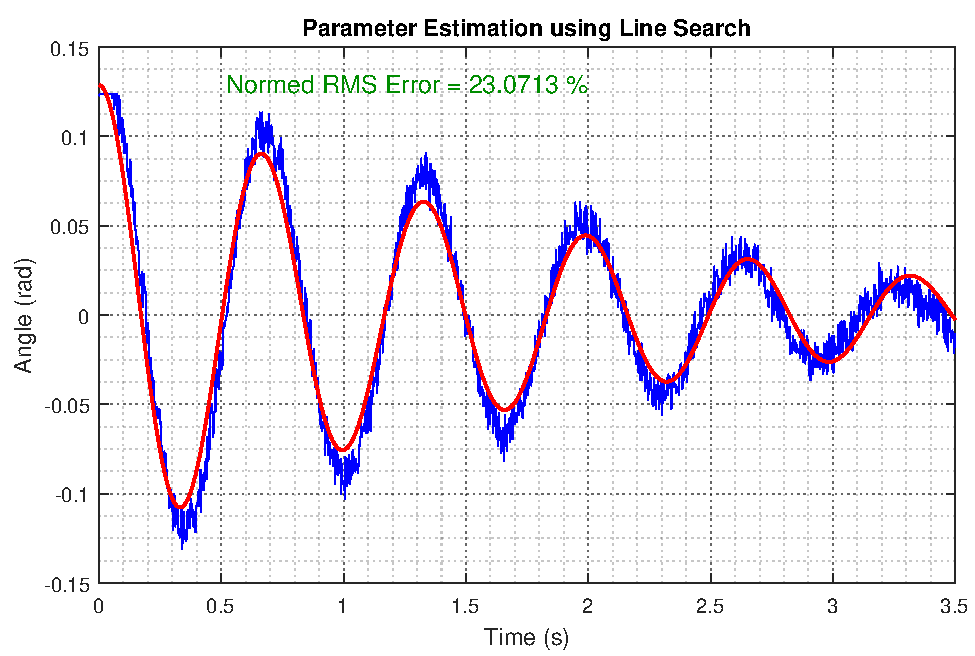
\includegraphics[scale=.55]{figures/ErrorNoEndLineSearch}
	\captionof{figure}{Normed RMS Error removing the last part of the data, using the parameters that Line Search gives}
	\label{ErrorNoEndLineSearch}
\end{figure}
%
\begin{figure}[H]
		\centering
	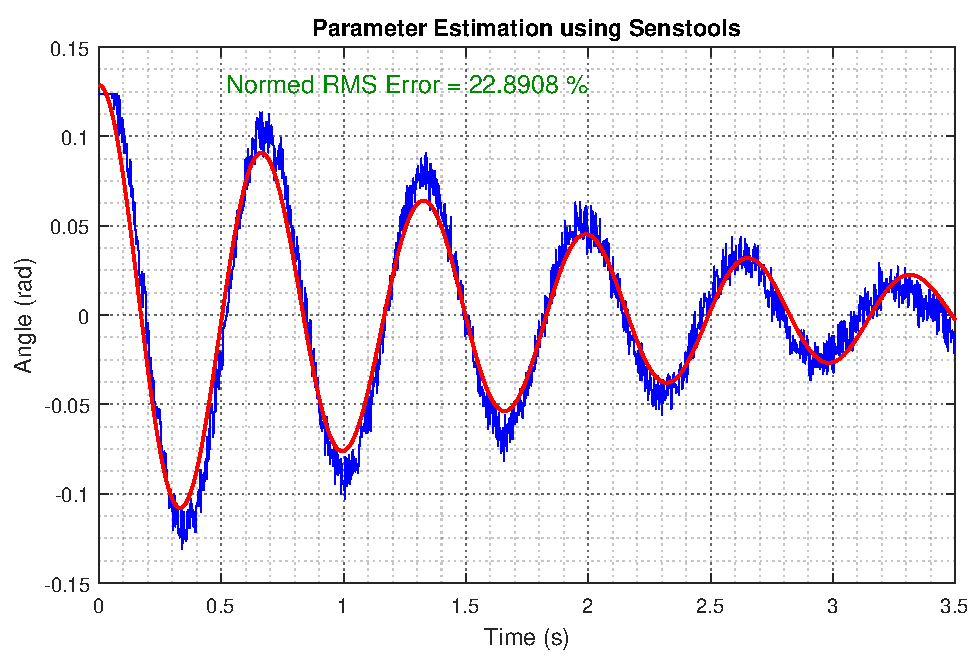
\includegraphics[scale=.55]{figures/ErrorNoEndSenstools}
	\captionof{figure}{Normed RMS Error removing the last part of the data, using the parameters that Senstools gives}
	\label{ErrorNoEndSenstools}
\end{figure}